\documentclass[11pt]{amsart}
%prepared in AMSLaTeX, under LaTeX2e
\addtolength{\oddsidemargin}{-.55in} 
\addtolength{\evensidemargin}{-.55in}
\addtolength{\topmargin}{-.2in}
\addtolength{\textwidth}{1.0in}
\addtolength{\textheight}{.4in}

\renewcommand{\baselinestretch}{1.1}

\usepackage{verbatim,fancyvrb}

\usepackage{palatino,amssymb}

\usepackage{tikz}
\usetikzlibrary{arrows.meta}

\newtheorem*{thm}{Theorem 16.0}
\newtheorem*{defn}{Definition}
\newtheorem*{example}{Example}
\newtheorem*{problem}{Problem}
\newtheorem*{remark}{Remark}

\newcommand{\mtt}{\texttt}
\usepackage{alltt,xspace}
\newcommand{\mfile}[1]
{\medskip\begin{quote}\scriptsize \begin{alltt}\input{#1.m}\end{alltt} \normalsize\end{quote}\medskip}

%\usepackage[final]{graphicx}

\usepackage[pdftex, colorlinks=true, plainpages=false, linkcolor=blue, citecolor=red, urlcolor=blue]{hyperref}

% macros
\newcommand{\bc}{\mathbf{c}}
\newcommand{\br}{\mathbf{r}}
\newcommand{\bv}{\mathbf{v}}
\newcommand{\bx}{\mathbf{x}}
\newcommand{\by}{\mathbf{y}}

\newcommand{\CC}{\mathbb{C}}
\newcommand{\RR}{\mathbb{R}}
\newcommand{\ZZ}{\mathbb{Z}}

\newcommand{\eps}{\epsilon}
\newcommand{\grad}{\nabla}
\newcommand{\lam}{\lambda}
\newcommand{\lap}{\triangle}

\newcommand{\ip}[2]{\ensuremath{\left<#1,#2\right>}}

%\renewcommand{\det}{\operatorname{det}}
\newcommand{\onull}{\operatorname{null}}
\newcommand{\rank}{\operatorname{rank}}
\newcommand{\range}{\operatorname{range}}

\newcommand{\prob}[1]{\bigskip\noindent\textbf{#1.}\quad }
\newcommand{\exer}[2]{\prob{Exercise #2 in Lecture #1}}

\newcommand{\pts}[1]{(\emph{#1 pts}) }
\newcommand{\epart}[1]{\medskip\noindent\textbf{(#1)}\quad }
\newcommand{\ppart}[1]{\,\textbf{(#1)}\quad }

\newcommand{\Matlab}{\textsc{Matlab}\xspace}
\newcommand{\Octave}{\textsc{Octave}\xspace}
\newcommand{\Python}{\textsc{Python}\xspace}

\DefineVerbatimEnvironment{mVerb}{Verbatim}{numbersep=2mm,
frame=lines,framerule=0.1mm,framesep=2mm,xleftmargin=4mm,fontsize=\footnotesize}

\newcommand{\ema}{\emach}
\newcommand{\emach}{\eps_{\!_{\text{m}}}}


\begin{document}
\scriptsize \noindent Math 661 Optimization (Bueler) \hfill 29 August, 2016
\normalsize

\medskip\bigskip
\Large
\centerline{Five example optimization problems}

\bigskip\medskip
\normalsize

\thispagestyle{empty}

There are three goals in starting the course with examples:
\renewcommand{\labelenumi}{\arabic{enumi})}
\begin{enumerate}
\item To suggest how optimization can come from real-world applications.
\item To allow you to create, for yourself, some of the basic theoretical and numerical ideas for how to solve such problems.
\item To provide examples on which to practice/learn \Matlab/\Octave\footnote{You may use other languages such as \Python, but I will only provide \Matlab/\Octave examples and solutions.} programming.
\end{enumerate}
While the textbook\footnote{J.~Nocedal \& S.~Wright, \emph{Numerical Optimization}, 2nd ed., 2006} does not give any fleshed-out examples, the authors, and other such experts, have of course been exposed to many of them.

Regarding goal 2), your method may be ``brute force'' or inefficient \dots \emph{that is just fine!}  The textbook and the rest of the content of the course will make more sense if you see that brute force approaches are the starting point of later elegant algorithms.

Assignment \#1 is based on these examples, but this document does not address how to solve these optimization problems.  Note that each example has a ``code name'' like ``\texttt{fit}.''  I will alse use this to name my corresponding \Matlab code (e.g.~``\texttt{fit.m}'') when I hand out solutions to A \#1.

Later Assignments will be largely based on textbook exercises, but I'll add my own problems and examples when needed.

\bigskip
\renewcommand{\labelenumi}{\Roman{enumi}. \quad}
\begin{enumerate}
\item (\texttt{calcone})  \quad Let
    $$f(x) = \left(x^2 + \cos x\right)^2 - 10 \sin(5 x).$$
Compute
    $$\min_{x\in [0,2]} f(x)$$

You may write the same problem as an inequality-constrained optimization in form (1.1), on page 3 of the textbook, namely as
	$$\min_{x\in\RR} f(x) \qquad \text{subject to }\quad \begin{matrix} x \ge 0 \\ 2 - x \ge 0\end{matrix}$$
In this standard form, $\mathcal{E}=\emptyset$, $\mathcal{I}=\{1,2\}$, $c_1(x)=x$, and $c_2(x)=2-x$.  However, I assert no particular benefit to this standardized form in this case.

You saw such problems in Calculus I.  This one is hard to do by hand; it benefits from some programming and visualization using \Matlab.  Start your solution by plotting $f(x)$ on the given interval; you'll know something close to the solution just from that picture.


\medskip
\item (\texttt{fit})  \quad Consider the following 11 data which are plotted below:

\bigskip
\begin{tabular}{c|ccccccccccc}
x & 0.000 & 0.100 & 0.200 & 0.300 & 0.400 & 0.500 & 0.600 & 0.700 &  0.800 &  0.900 &  1.000 \\
\hline
y & 4.914 & 3.666 & 2.289 & 1.655 & 1.029 & 0.739 & 0.393 & 0.090 & -0.197 & -0.721 & -0.971
\end{tabular}

\bigskip
\begin{center}
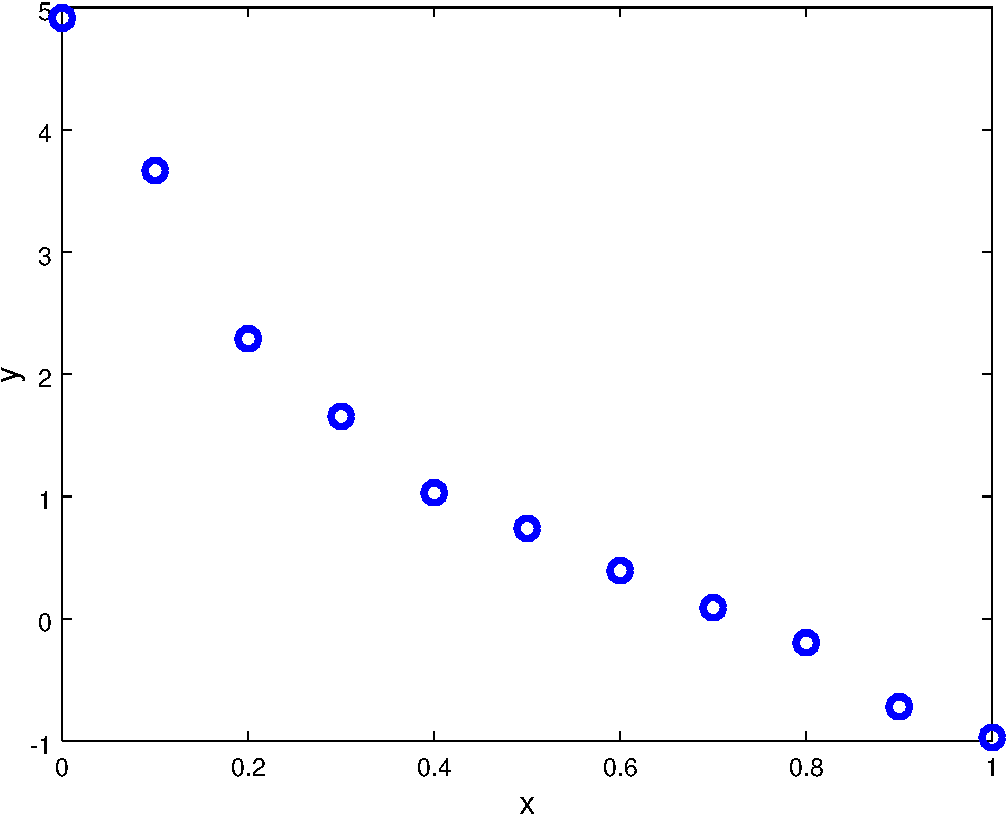
\includegraphics[width=0.5\textwidth]{fitdata}
\end{center}

\medskip
Suppose we believe that this data can be fit by a function of the for $g(x) = c_1 + c_2 x + c_3 e^{-5 x}$.  If the sense of ``fit'' is that the sum of the squares of the misfits should be as small as possible then we would solve
	$$\min_{c \in \RR^3} f(c)$$
where we define the objective function to be
	$$f(c) = \frac{1}{2} \sum_{j=1}^{11} \left(g(x_j) - y_j\right)^2 = \frac{1}{2} \sum_{j=1}^{11} \left(c_1 + c_2 x_j + c_3 e^{-5 x_j} - y_j\right)^2.$$

This problem is already in form (1.1) from the textbook, with $c = \left[c_1,c_2,c_3\right]$ an unknown vector of coefficients in $\RR^3$, and with no constraints ($\mathcal{E}=\emptyset,\mathcal{I}=\emptyset$).  Here $x_j,y_j$ are the data, with $x_j = 0.1 (j-1)$ regularly-spaced.  Note we are \emph{not} finding $x_j$ or $y_j$ values in the minimization process; these values merely determine the objective function.  Also note that the overall factor of $1/2$ in defining the function $f(\bc)$ is just a convenience for differentiating.\footnote{\dots a hint about the standard algorithms for finding the minimum.}

\medskip
\item (\texttt{salmon})  \quad Ed and Thomas caught 21 salmon, and all will be filleted.  Of these, $x_1$ will be eaten fresh, which requires 2 time units per fish.  Then $x_2$ will be vacuum-packed and frozen (3 time units per fish) and another $x_3$ will be smoked, vacuum-packed, and frozen (4 time units per fish).  Thus the total amount of processing time is $2 x_1 + 3 x_2 + 4 x_3$.  However, at most 2 fish can be eaten fresh before they go bad, and at most 10 fish can be smoked in the time allowed.

Finding $x_1,x_2,x_3$ to minimize the total processing time means solving this constrained problem with $f(x) = 2 x_1 + 3 x_2 + 4 x_3$:
	$$\min_{x\in\RR^3} f(x) \qquad \text{subject to }\quad \begin{matrix} x_1 + x_2 + x_3 = 21 \\ 0 \le x_1 \le 2 \\ 0 \le x_2 \\ 0 \le x_3 \le 10 \end{matrix}$$
This problem is not in standard form (1.1), but an easy exercise on A \#1 asks you to put all of the inequality constraints into the form ``$c_i(x) \ge 0$'' to make it so.

\medskip
\item (\texttt{tsp})  \quad Jill sells amazing devices which make your brain absorb math more easily.  To sell these devices she plans to visit cities A, F, J, N, W starting and ending at city S.  Some pairs of cities have connecting flights and some do not; the one-way costs of the various flights are shown below in a \emph{graph} with costs (``weights'') on each connection (``edge'').  It is clear to Jill that she should visit each city exactly once, except for returning to S at the end.  Note that a possible itinerary is expressible as a seven-letter string like ``SANFWJS.''

\vspace{-5mm}
\begin{tikzpicture}[scale=0.9]
\begin{scope}[every node/.style={circle,thick,draw}]
    \node (A) at (-0.5,0) {A};
    \node (F) at (0,3)    {F};
    \node (J) at (2,-1)   {J};
    \node (N) at (-3,3)   {N};
    \node (S) at (3,-3)   {S};
    \node (W) at (3,1)    {W} ;
\end{scope}

\begin{scope}[every node/.style={fill=white},
              every edge/.style={draw=black,very thick}]
    \path (A) edge node {$100$} (F);
    \path (A) edge node {$100$} (J);
    \path (A) edge node {$150$} (N);
    \path (A) edge[bend right=50] node {$250$} (S);
    \path (A) edge node {$150$} (W);
    %\path (F) edge node {$150$} (J);
    \draw[very thick] (F.east) .. controls (3,4) and (6,0) .. (J.east) node[midway] {$150$};
    \path (F) edge node {$200$} (N);
    %\path (F) edge node {$300$} (S);
    \draw[very thick] ([yshift=3mm,xshift=-1mm] F.east) .. controls (4,5) and (7,-1) .. (S.east) node[midway] {$300$};
    \path (F) edge node {$250$} (W);
    \path (J) edge node {$200$} (S);
    \path (J) edge node {$200$} (W);
\end{scope}
\end{tikzpicture}

\medskip
This is an example of the famous \emph{traveling salesperson problem}.  If $x$ denotes a feasible seven-letter string (itinerary) then we may define the objective function $f(x)$ to be the cost of that itinerary; thus $f(x)$ is defined using the edge weights.  Finding a feasible itinerary is generally nontrivial---it corresponds to finding a \emph{Hamiltonian cycle}---in fact one may add in all remaining edges with large weights so that any itinerary $x$ is feasible with well-defined cost $f(x)$.

The problem \emph{could} be written
	$$\min_{x \text{ is feasible itinerary}} f(x)$$
but this does \emph{not} mean it is in standard form (1.1) because there is no sensible way to treat the possible inputs as ``$x \in \RR^n$.''  This is a \emph{discrete optimization} problem, not a continuous problem as covered in form (1.1) and the textbook generally.

\medskip
\item (\texttt{beam})  \quad A new tent design requires bending a pole to go from one corner of the tent to another while also having certain heights at particular locations.  Note that the corners of the tent, and thus the ends of the pole, are on the ground.  We want to know the shape of the pole, which is modeled as a \emph{beam} in standard engineering language, so that fabric can be cut to reach the pole and yet be taut below it.

To be specific, the length of the tent along the ground is $\pi$ length units.  We seek a function $y=h(x)$, defined on the interval $x\in[0,\pi]$, for the height of the pole above the ground.  This function must be at least twice-differentiable and satisfy $h(0)=0$ and $h(\pi)=0$.  The theory of beams says that actual bent shape will be the minimizing solution $h$ of
    $$\min_h I[h]$$
where
    $$I[h] = \frac{1}{2} \int_0^\pi |h''(x)|^2\,dx$$
is called the objective \emph{functional}.  The input $h$ is itself a function from an (infinite-dimensional) vector space of functions.

The following particular inequalities, shown in the figure below, give locations where the heights are constrained:
\begin{align*}
0.9 &\le h(1) \le 1.1 \\
1.2 &\le h(2) \le 1.4 \\
0.4 &\le h(3) \le 0.6
\end{align*}

The figure does not show the shape of the tent pole.  That is, it does not show the \emph{solution} of the minimization problem.  That solution, after all, has minimal concavity, i.e.~size of second derivative, subject to the constraints.  The figure does, however, show a \emph{feasible} $h(x)$ which has the required differentiability, satisfies $h(0)=h(\pi)=0$, and satisfies the inequality constraints.

\bigskip
\begin{center}
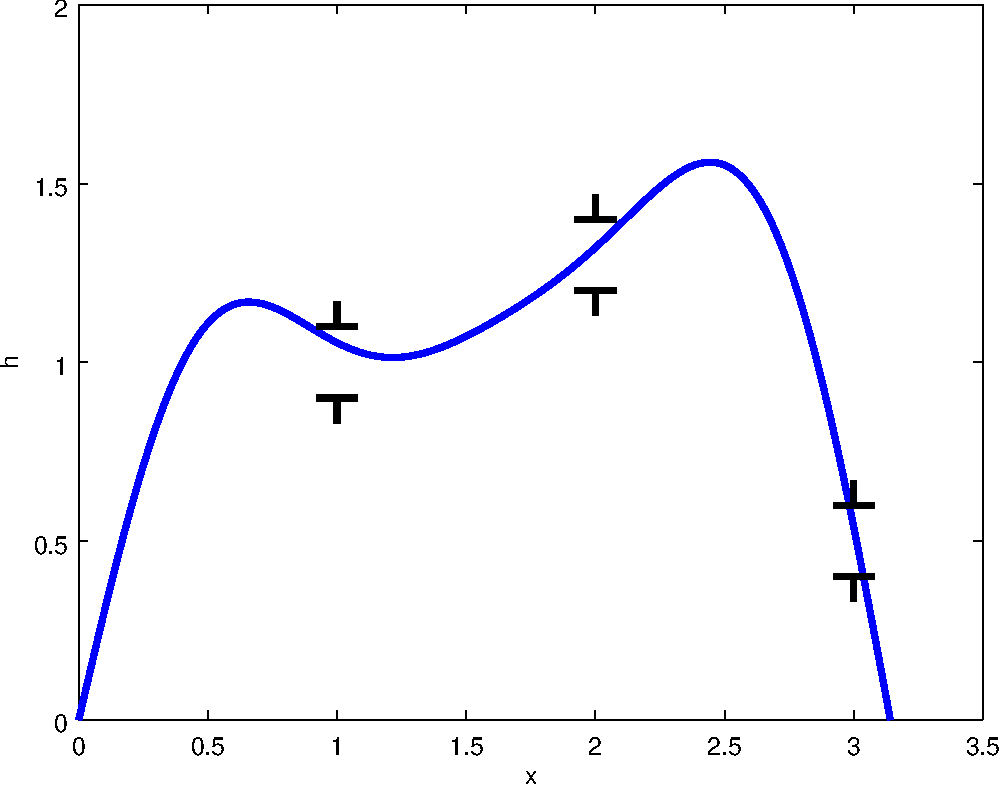
\includegraphics[width=0.6\textwidth]{beamgates}
\end{center}

\end{enumerate}

\end{document}

